\ifcase0  % choose 0=slides, 1=article, 2=refart
   \documentclass[aspectratio=169,ignorenonframetext,12pt]{beamer}
\or\documentclass[a4paper,11pt]{article}
   \usepackage{url,beamerarticle}
\or\documentclass[a4paper,11pt]{refart}
   \let\example\relax
   \usepackage{url,beamerarticle}
\fi

\ifcase0  % choose a theme like these
   \usetheme{Goettingen}% I recommend
\or\usetheme{Singapore}
\or\usetheme{Boadilla}
\or\usetheme{Pittsburgh}
\or\usetheme{Madrid}
\or\usetheme{Warsaw} % common choice, but often poor
\fi

\usepackage{graphicx,pgfplots,parskip}



\title{Simple `beamer' template for presentations} 
\author{Prof Tony Roberts\\
The University of Adelaide}
\date{29 April 2019}


\begin{document}

\begin{frame}
\maketitle
\end{frame}


\begin{abstract}
This abstract, being outside the frame environment, does not appear in the presentation.  Your outline will be the basis for a couple of sentences of talk for each of the following questions:
\begin{itemize}
\item What was done?
\item Why do it?
\item What were the results?
\item What do the results mean in theory and/or practise?
\item What is the reader's benefit?
\item How can the readers use this information for themselves? 
\end{itemize}
\end{abstract}


\begin{frame}{Outline}
\tableofcontents
\end{frame}



\section{Present notes, not a discourse}
Using section and subsection commands, outside of frames, provides a table of contents and progress information to beamer.
\begin{frame}{Present notes, not a discourse}

Aim for five to ten slides for a 25~minute presentation.

Certainly no more than 15.

Use a note form for the content of each slide.

\begin{theorem}
Mathematics works within the Beamer class, $\exp(i\pi)+1=0$\,, including theorems.
\end{theorem}

Click: \url{http://www.maths.adelaide.edu.au} 
\end{frame}



\section{Divide your presentation into frames}
\begin{frame}{Divide your presentation into frames}

In the Beamer documentclass, include the text you wish to show within a \texttt{frame} environment.

Material you put outside of \texttt{frame} environments will not appear.

However, as in the preamble, the package \texttt{beamerarticle} empowers this document to be typeset in its entirety, including the non-framed material.

Typeset the presentation using \texttt{pdflatex}.
\end{frame}



\section{Prefer titles that make a statement}
\begin{frame}{Prefer titles that make a statement}

Many opt for meaningless titles and section titles.  

Instead, make titles convey information.

\pause

Use \texttt{pause} commands almost anywhere to progressively step through material.

\pause

\begin{figure}
\centering
\caption{Figure and table environments also work.
Use \texttt{includegraphics} or \texttt{pgfplots}.}
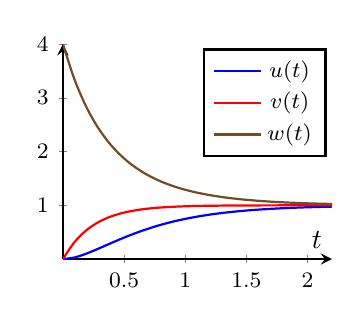
\begin{tikzpicture}
\begin{axis}[footnotesize,axis lines=middle
,xlabel={$t$},no marks,thick,domain=0:2.2,smooth ]
\addplot+[]{1-2*exp(-2*x)+exp(-4*x)};
\addlegendentry{$u(t)$};
\addplot+[]{1-exp(-4*x)};
\addlegendentry{$v(t)$};
\addplot+[]{1+2*exp(-2*x)+exp(-4*x)};
\addlegendentry{$w(t)$};
\end{axis}
\end{tikzpicture}
\end{figure}

\end{frame}




\section{Conclusion}
\begin{frame}{Conclusion}

Finish with your conclusions displayed: \emph{not} a list of references, \emph{nor} a meaningless ``thank you'' slide.

\vfill
\begin{quote}
	Three rules of public speaking: Be forthright.  Be brief.  Be
	seated. \hfill(S. Dressel \& J. Chew, 1987)
\end{quote}
\end{frame}




\end{document}

